\section{Оборудование и инструментальные погрешности}
\begin{figure}[ht!]
    \centering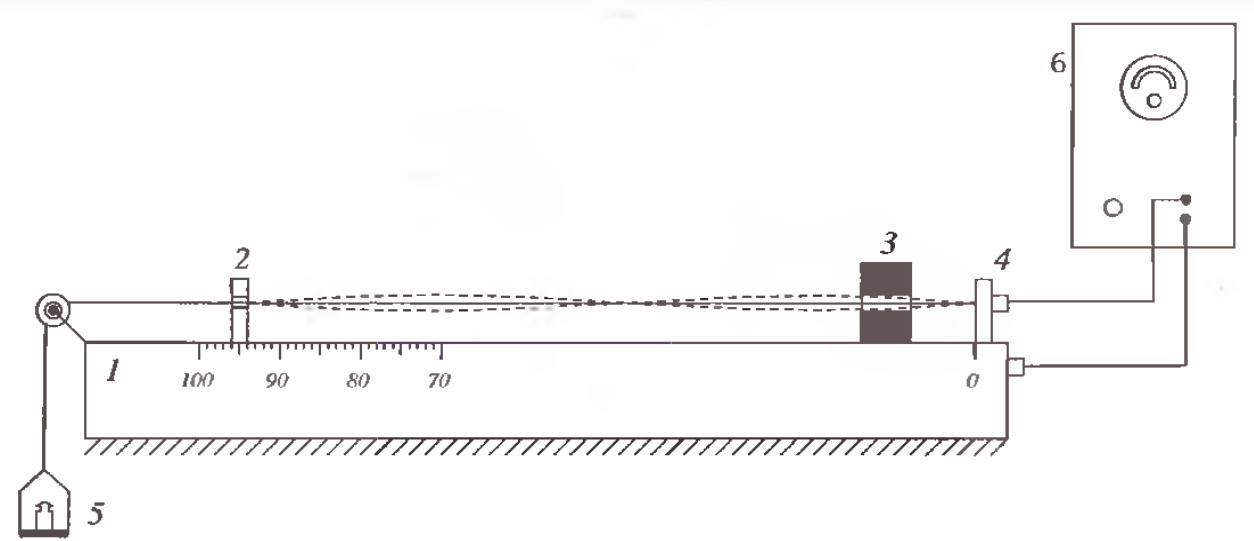
\includegraphics[width=0.8\linewidth]{img/img1.png}
\end{figure}

Схема установки изображена на рисунке. На массивной рейке 1 установлены опора 2 и магнит 3,
которые можно перемещать вдоль рейки, а также неподвижная опора 4. Один конец струны
закреплён в изоляторе опоры 4. От него струна проходит между полюсами магнита и через
опору 2, которая дает возможность струне перемещаться в горизонтальном направлении,
неподвижный блок и соединяться с чашкой 5, на которую помещают грузы. Такое устройство
необходимо для натяжения струны. К концу струны, закреплённому в изоляторе опоры 4, и к
массивной рейке 1 подводится переменное напряжение от звукового генератора 6. Движение
струны вызывается силой Ампера, действующей на проводник с током в магнитном поле. Частота
действия силы, раскачивающей струну, равна частоте генератора.

Сила Ампера не только возбуждает колебания, но и поддержтивает их.
Поток энергии  распространяется по всей струне. Однако в чисто стоячей волне распространение
энергии невозможно, поэтому узлы размываются. Коэффициент бегучасти должен быть много меньше 1:
\[\frac{A_1-A_2}{A_2}\ll 1\]

$A_1$~--- амплитуда падающей волны, $A_2$~--- амплитуда отражённой волны.
Величина $A_1-A_2$ равна половине величины размытия узлов. Амплитуда в пучности равна $2A_2$.

Если это соотношение выполняется недостаточно хорошо, то надо уменьшить величину подводимой мощности.

Действие силы Ампера должно привести к поляризации колебаний в плоскости, перпендикулярной
направлению магнитного поля. В реальности это не всегда так.
